\textbf{Máster Universitario en Economía. Microeconomía Avanzada. Curso 23/24. Ejercicios 2}
\begin{center}
    \textbf{Paredes Aguilera Christian Limbert}
\end{center}
\begin{center}
	\rule{1\textwidth}{0.4pt}
\end{center}


\begin{enumerate}[\textbf{Ejercicio} \bfseries 1.]

    % -------------------- 1.
    \item  \textbf{Considere el axioma de Transferencia Asignaciones Proporcionales. Muestre de manera gráfica, cómo la dirección final de las transferencias entre dos agentes depende de la distribución de la dotación inicial.}\\

	\textbf{Solución:}
	\begin{center}
	    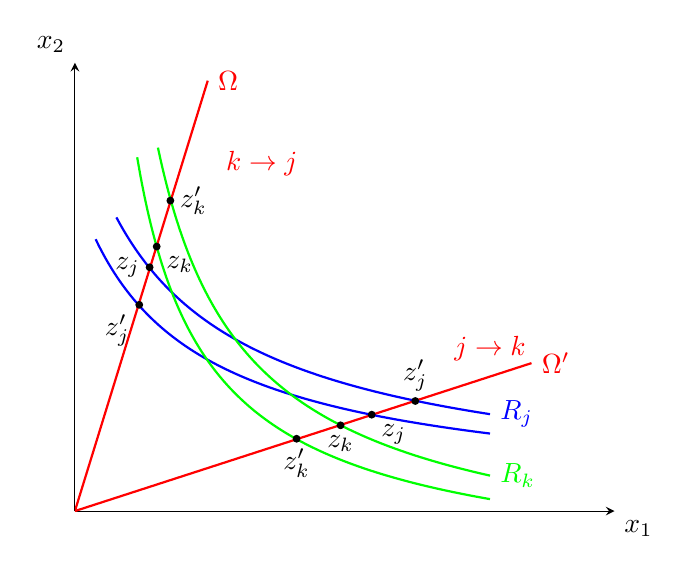
\begin{tikzpicture}
		\begin{axis}[
		    xmin=0, xmax=1.3,
		    ymin=0, ymax=4,
		    axis lines=center,
		    xlabel={$x_1$}, ylabel={$x_2$},
		    xtick=\empty, ytick=\empty,
		    xlabel style={below right},
		    ylabel style={above left}
		]

		\addplot[domain=0:1.1, samples=100, smooth, thick, red] {1.2*x}node[right]{$\Omega'$};
		\addplot[domain=0:.32, samples=100, smooth, thick, red] {12*x}node[right]{$\Omega$};

		\addplot[domain=.1:1, samples=100, smooth, thick, blue] {pow(x+.2,-0.8)}node[right]{$R_j$};
		\addplot[domain= .05:1, samples=100, smooth, thick, blue] {.8*pow(x+.2,-0.8)};

		\addplot[domain=.2:1, samples=100, smooth, thick, green] {pow(x-.02,-0.8)-.7}node[right]{$R_k$};
		\addplot[domain=.15:1, samples=100, smooth, thick, green] {.8*pow(x-.01,-0.8)-.7};

		\addplot[mark=*,mark size=1.2pt] coordinates {(0.23,2.77)}node[right]{$z_k'$};
		\addplot[mark=*,mark size=1.2pt] coordinates {(0.197,2.36)}node[below right]{$z_k$};
		\addplot[mark=*,mark size=1.2pt] coordinates {(0.18,2.175)}node[left]{$z_j$};
		\addplot[mark=*,mark size=1.2pt] coordinates {(0.155,1.84)}node[below left]{$z_j'$};

		\addplot[mark=*,mark size=1.2pt] coordinates {(.82,.982)}node[above]{$z_j'$};
		\addplot[mark=*,mark size=1.2pt] coordinates {(.715,.86)}node[below right]{$z_j$};
		\addplot[mark=*,mark size=1.2pt] coordinates {(.64,.765)}node[below]{$z_k$};
		\addplot[mark=*,mark size=1.2pt] coordinates {(.534,.645)}node[below]{$z_k'$};

		\addplot[red] coordinates {(1,1.645)}node[below]{$j\to k$};
		\addplot[red] coordinates {(.45,3.3)}node[below]{$k\to j$};

		\end{axis}
	    \end{tikzpicture}
	\end{center}
	\vspace{.5cm}

    % -------------------- 2.
    \item \textbf{\boldmath Suponga una economía con dos agentes $(j \textbf{ y } k)$ y dos bienes $(1 \textbf{ y } 2)$ en la cual las dotaciones iniciales son $\omega_j = (8, 2)$ y $\omega_k = (2, 8)$. Si las preferencias de $k$ vienen definidas por la función $u_k(x_1, x_2) = x_1^{1/2}x_2^{1/2}$ ¿en qué dirección iría la transferencia de recursos según el axioma de Transferencia Asignaciones-Proporcionales en cada uno de los siguientes escenarios?}
	\begin{enumerate}[\bfseries i)]

	    % ---------- i)
	    \item \textbf{\boldmath $u_j^0(x_1,x_2) = x_1^{1/2}x_2^{1/2}$}. Para graficar la curva, reemplazamos $\omega_j=(8,2)$ tal que, 
		$$u=8^{1/2}2^{1/2}=4.$$ 
		Entonces, la curva de indiferencia de $j$ será:
		$$x_2=\dfrac{4^2}{x_1}.$$

	    % ---------- ii)
	    \item \textbf{\boldmath $u_j^1(x_1,x_2) = x_1^{3/4}x_2^{1/4}$}. Para graficar la curva, reemplazamos $\omega_j=(8,2)$ tal que,
		$$u=8^{3/4}\cdot 2^{1/4}.$$
		Entonces, la curva de indiferencia de $j$ será:
		$$x_2=\dfrac{8^{3/4}\cdot 2^{1/4}}{x_1^3}.$$


	    % ---------- iii)
	    \item \textbf{\boldmath $u_j^2(x_1,x_2) = x_1^{1/4}x_2^{3/4}$}. Para graficar la curva, reemplazamos $\omega_j=(8,2)$ tal que,
		$$u=8^{1/4}\cdot 2^{3/4}.$$
		Entonces, la curva de indiferencia de $j$ será:
		$$x_2=\dfrac{8^{1/4}\cdot 2^{3/4}}{x_1^3}.$$

	\end{enumerate}

	GRÁFICA

	\begin{center}
	    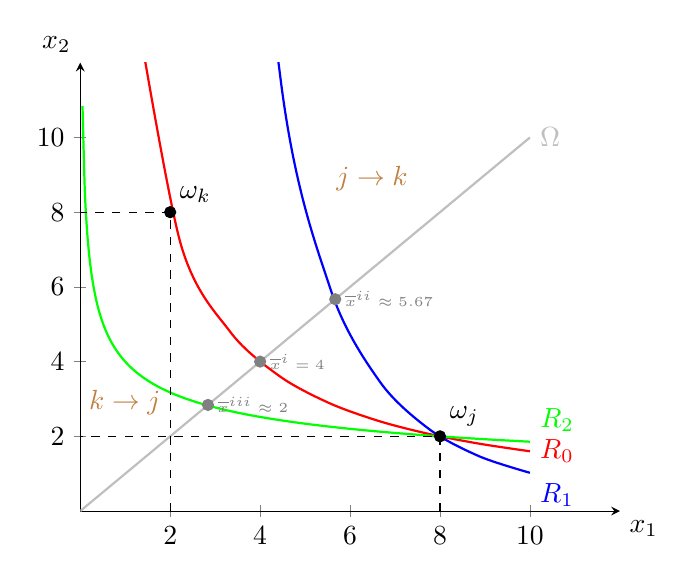
\begin{tikzpicture}
		\begin{axis}[
		    xmin=0, xmax=12,
		    ymin=0, ymax=12,
		    axis lines=center,
		    xlabel={$x_1$}, ylabel={$x_2$},
		   xtick={0,2,...,10}, ytick={0,2,...,10},
		    xlabel style={below right},
		    ylabel style={above left}
		]

		\addplot[domain=0:10, samples=10, smooth, thick, red] {(4^2)/x}node[right]{$R_0$};
		\addplot[domain=0:10, samples=10, smooth, thick, blue] {(8^(3/4)*2^(1/4))^4/x^3}node[below right]{$R_1$};
		\addplot[domain=0:10, samples=200, smooth, thick, green] {((8^(1/4)*2^(3/4))^4/x)^(1/3)}node[above right]{$R_2$};
		\addplot[domain=0:10, samples=10, smooth, thick, gray!50] {x}node[right]{$\Omega$};

		\draw[dashed] (axis cs:8,0) -- (axis cs:8,2) -- (axis cs:0,2);
		\addplot[black,mark=*,mark size=2pt] coordinates {(8,2)}node[above right]{$\omega_j$};
		\draw[dashed] (axis cs:2,0) -- (axis cs:2,8) -- (axis cs:0,8);
		\draw[dashed,brown] (axis cs:8,2)(axis cs:2,3.5)node[below left]{$k\to j$};
		\draw[dashed,brown] (axis cs:8,2)(axis cs:7.5,9.5)node[below left]{$j\to k$};
		\addplot[black,mark=*,mark size=2pt] coordinates {(2,8)}node[above right]{$\omega_k$};

		\addplot[black,mark=*,mark size=2pt,gray] coordinates {(4,4)}node[right]{\tiny$\overline{x}^i=4$};
		\addplot[black,mark=*,mark size=2pt,gray] coordinates {(5.67,5.67)}node[right]{\tiny$\overline{x}^{ii}\approx 5.67$};
		\addplot[black,mark=*,mark size=2pt,gray] coordinates {(2.84,2.84)}node[right]{\tiny$\overline{x}^{iii}\approx 2$};


		\end{axis}
	    \end{tikzpicture}
	\end{center}
	\vspace{.5cm}

	Sabemos que las asignaciones proporcionales son $x_1=x_2$. De donde, 
	$$x_1^\alpha\cdot x_2^{1-\alpha}=\overline{x}.$$
	Por lo tanto,
	\begin{enumerate}[\bfseries i.]
	    \item  $\overline{x}^i=8^{1/2}\cdot 2^{1/2}=4$ (No existe transferencia, dado que la sociedad indica que las situaciones son iguales).
	    \item $\overline{x}^{ii}=8^{3/4}\cdot 2^{1/4}\approx 5.67$. (La transferencia iría de $j$ a $k$). Ya que $j$ es mejor que $k$.
	    \item $\overline{x}^{iii}=8^{1/4}\cdot 2^{3/4}\approx 2.84$. (La transferencia iría de $k$ a $j$). Ya que $k$ es mejor que $j$ o $j$ es peor que $k$.
	\end{enumerate}
	\vspace{.5cm}


    % -------------------- 3.
    \item \textbf{\boldmath Considere una economía con dos bienes, y una SOF que, para un precio exógenamente dado $\overline{p} \in \mathbb{R}^2_{++}$, tiene como objetivo maximizar el conjunto presupuestario más pequeño. Describa formalmente el principio de transferencias que permitiría al planificador llegar a estas preferencias sociales. ¿Cuál sería la idea normativa detrás de este principio de transferencias?}\\

	\textbf{Solución:} En este contexto, estamos analizando una economía con dos bienes y una Función de Orden Social (SOF) que aspira a maximizar el conjunto presupuestario más reducido para un precio dado de manera exógena $\overline{p} \in \mathbb{R}^2_{++}$.

	Primero, establecemos el conjunto viable como $B(p, z) = \{x \in \mathbb{R}^2_{+} | px \leq pz\}$. Este conjunto engloba todas las asignaciones posibles que son factibles dada la asignación $z$ y el precio $p$.

	A continuación, introducimos un axioma que nos permitirá alcanzar las preferencias sociales deseadas. Este axioma establece que para todo $e \in E$ y $z_N , z'_N \in \mathbb{R}^n$, si existen $j, k \in N$ tal que:
	$$pz'_j > pz_j > pzk > pz'_k$$
	$$z_j \in \max |R_j B(p, z_j ),$$ 
	$$z'_j \in \max|R_j B(p, z'_j),$$
	$$zk \in \max |R_k B(p, zk),$$ 
	$$z'_k \in \max |R_k B(p, z'_k),$$ 
	Donde, $zi = z'_i$ para todo $i \neq \{j, k\}$; entonces $z_N \textbf{R}(e)z'_N$.

	Este axioma tiene como objetivo minimizar la desigualdad entre los conjuntos factibles o de oportunidad. La idea es que si es posible realizar una transferencia de recursos de $z'_N$ a $z_N$ de tal manera que el conjunto presupuestario de $z_N$ se reduzca sin aumentar el de $z'_N$, entonces la sociedad preferirá realizar esa transferencia.

	La idea normativa detrás de este principio de transferencias es la de eficiencia y equidad. Al maximizar el conjunto presupuestario más pequeño, el planificador está buscando asegurar que los recursos se utilicen de la manera más eficiente posible. Al mismo tiempo, al minimizar la desigualdad entre los conjuntos factibles, el planificador está promoviendo una distribución más justa de los recursos.\\\\

    % -------------------- 4.
    \item \textbf{Considere la economía y las dos asignaciones sociales representadas en el siguiente gráfico. ¿Cuál sería el ranking social de estas asignaciones si el planificador aboga por asumir Transferencia Asignaciones-Proporcionales? ¿Cuál sería la idea detrás del ranking resultante?.}\\

	\textbf{Solución:} En este escenario, estamos considerando una economía con dos asignaciones sociales representadas en un gráfico. Estamos interesados en determinar el ranking social de estas asignaciones si el planificador aboga por asumir Transferencia Asignaciones-Proporcionales.

La sociedad establece que $z_N \textbf{R}(\epsilon)z'_N$. Esto significa que, en el orden social, la asignación $z_N$ es preferida o al menos no es peor que $z'_N$. En otras palabras, la sociedad preferiría una mayor igualdad en la distribución de los dos bienes.

Esta preferencia no solo depende de la dotación inicial $\Omega$, sino también de las formas de las curvas de indiferencia (CI’s). Las curvas de indiferencia representan las combinaciones de bienes que proporcionan el mismo nivel de satisfacción al individuo.

Si la curva de indiferencia que pasa por $z_k'$ fuera un poco más inclinada, el orden social sería el inverso. Esto se debe a que en ese caso el individuo daría más valor a las cestas que incluyen mucho del bien $x_1$.

En resumen, el ranking social de las asignaciones depende tanto de las preferencias de la sociedad por la igualdad como de las preferencias individuales reflejadas en las curvas de indiferencia. La idea detrás del ranking resultante es equilibrar estas dos consideraciones para lograr una distribución de bienes que sea tanto equitativa como eficiente.\\\\


    % -------------------- 5.
    \item \textbf{Responda a las siguientes preguntas sobre las asignaciones sociales representadas en la gráfica adjunta:}
	\begin{enumerate}[\bfseries i)]

	    % ---------- i)
	    \item  \textbf{\boldmath ¿Cuál es el orden social en base a la SOF $\textbf{R}^{slex}$?.}\\

		\textbf{Solución:} En este orden, un vector de asignación $z'_N$ se prefiere a otro $z_N$ si la probabilidad de que un individuo aleatorio esté mejor en $z'_N$ que en $z_N$ es mayor. Es decir, $z'_N\textbf{R}(\epsilon)z_N$.\\

	    \item \textbf{Suponga ahora que la productividad marginal de referencia viene dada por la linea discontinua roja. En este caso, ¿cuál sería el orden social de las mismas dos asignaciones sociales? ¿Qué sucedería en este caso?}\\

		\textbf{Solución:} En este escenario, donde la productividad marginal de referencia está representada por la línea discontinua roja, estamos evaluando el orden social entre dos asignaciones sociales específicas utilizando la SOF $\textbf{R}^{slex}$.

		Si tomamos $s' \in \mathbb{R}_+$ como nuestro único punto de referencia, encontramos que $z_N \textbf{R}^{slex}(\epsilon)z'_N$. Esto significa que, en el orden social $\textbf{R}^{slex}$, la asignación social $z_N$ es preferida o al menos no es peor que $z'_N$.

		La clave aquí es que la productividad de referencia es muy baja. En tales circunstancias, la sociedad tiende a dar más importancia a las personas con bajos ingresos. Esto se traduce en un beneficio para aquellos individuos que tienen una mayor preferencia por el ocio, ya que son más propensos a recibir una mayor asignación de recursos en este orden social.

		Este fenómeno puede ser interpretado como una forma de equidad en la distribución de recursos. En una sociedad donde la productividad de referencia es baja, aquellos con menores ingresos o mayor preferencia por el ocio son vistos como más necesitados o merecedores de recursos. Por lo tanto, el orden social $\textbf{R}^{slex}$ refleja esta prioridad al preferir la asignación $z_N$ sobre $z'_N$.\\\\

	    \end{enumerate}

    % -------------------- 6.
    \item \textbf{Utilice la siguiente tabla para demostrar que en un contexto de salud los axiomas normativos de Pareto Débil y de Transferencia Igual-Salud (una variante de Transferencia Salud Perfecta) son incompatibles entre si.}

    \begin{center}
	\begin{table}[h]
	    \centering
	    \begin{tabular}{|c|c|c|c|c|c|c|}
		\hline
		 & \multicolumn{3}{c|}{Ana} & \multicolumn{3}{c|}{Borja} \\
		\hline
		Asignación & Salud & Consumo & Preferencias & Salud & Consumo & Preferencias \\
		\hline
		1 & Malo & 9000 & 3 & Malo & 10000 & 1 \\
		2 & Malo & 9100 & 2 & Malo & 9900 & 4 \\
		3 & Bueno & 9000 & 1 & Bueno & 7900 & 3 \\
		4 & Bueno & 8900 & 4 & Bueno & 8000 & 2 \\
		\hline
	    \end{tabular}
	\end{table}
    \end{center}

	\textbf{Solución:} Consideremos dos asignaciones, la Asignación 1 y la Asignación 3, de la tabla. En la Asignación 1, tanto Ana como Borja se encuentran en un estado de salud “Malo”. En la Asignación 3, ambos individuos tienen un estado de salud “Bueno”.

Según el axioma de Transferencia Igual-Salud, la Asignación 3 es preferible a la Asignación 1, ya que mejora la salud de ambos individuos sin alterar su consumo.

Sin embargo, si consideramos las preferencias individuales de Ana y Borja, encontramos un conflicto. Ana prefiere la Asignación 1 a la Asignación 3, mientras que Borja prefiere la Asignación 3 a la Asignación 1.

De acuerdo con el axioma de Pareto Débil, no podemos afirmar que la Asignación 3 es preferible a la Asignación 1, ya que Ana prefiere la Asignación 1 a la Asignación 3.

Por lo tanto, encontramos una incompatibilidad entre los axiomas de Pareto Débil y de Transferencia Igual-Salud. Esta incompatibilidad surge debido a las diferencias en las preferencias individuales de Ana y Borja respecto a su estado de salud.


\end{enumerate}
